\documentclass[titlepage, 12pt]{book}
\usepackage[parfill]{parskip}
\usepackage{amsmath}
\usepackage{xcolor}
\usepackage{amsfonts}
\usepackage{setspace}
\usepackage{hyperref}
\usepackage{tcolorbox}
\usepackage{graphicx}
\graphicspath{ {./bin/} }
\tcbuselibrary{theorems}

\hypersetup{
    colorlinks=true,
    linkcolor=blue,
    filecolor=magenta,
    urlcolor=blue,
}

\DeclareMathOperator*{\argmax}{arg\,max}
\DeclareMathOperator*{\argmin}{arg\,min}

\newtcbtheorem[]{definition}{Definition}%
{colback=magenta!5,colframe=magenta!100!black,fonttitle=\bfseries}{th}

\newtcbtheorem[]{proposition}{Proposition}%
{colback=cyan!5,colframe=cyan!100!black,fonttitle=\bfseries}{th}

\newtcbtheorem[]{theorem}{Theorem}%
{colback=orange!5,colframe=orange!100!black,fonttitle=\bfseries}{th}

\newtcbtheorem[]{algorithm}{Algorithm}%
{colback=violet!5,colframe=violet!100!black,fonttitle=\bfseries}{th}

\newtcbtheorem[]{problem}{Problem}%
{colback=green!5,colframe=green!100!black,fonttitle=\bfseries}{th}

\begin{document}

\begin{titlepage}

	\raggedleft

	\vspace*{\baselineskip}

	{Bharathi Ramana Joshi\\\url{https://github.com/iambrj/notes}}

	\vspace*{0.167\textheight}

	\textbf{\LARGE Notes on competitive programming}\\[\baselineskip]

	\vfill

	\vspace*{3\baselineskip}

\end{titlepage}

\newpage

\tableofcontents

\chapter{Performance}

\begin{definition}{Operations per second}{}
    Most judges allow $10^8$ operations per second, but all allow $10^7$.
\end{definition}

Always pass arguments by reference when possible.

\chapter{Math}

\begin{definition}{Binet's formula for Fibonacci numbers}{}
    \begin{align*}
        f(n) = \frac{(1 + \sqrt{5}) ^ n - (1 - \sqrt{5}) ^ n}{2^n\sqrt{5}}
    \end{align*}
\end{definition}

\begin{theorem}{Fermat's little theorem}{}
  If $p$ is a prime then,
  \begin{align*}
    a^p = a\ (mod\ p)
  \end{align*}
  Therefore, if $a$ is not divisible by $p$, we can multiply both sides with
  $a^{-2}$ to find modular inverse efficiently:
  \begin{align*}
    a^{p - 2} = a^{-1}\ (mod\ p)
  \end{align*}
\end{theorem}

\chapter{Bitwise tricks}

\begin{algorithm}{xor of first $n$ natural numbers}{}
  \[ \begin{cases}
    n     & n \% 4 = 0 \\
    1     & n \% 4 = 1 \\
    n + 1 & n \% 4 = 2 \\
    0     & n \% 4 = 3
  \end{cases}
\]
\end{algorithm}

\begin{algorithm}{Minimum xor of pair in array}{}
  Sort and take min xor of adjacent elements.
\end{algorithm}

\chapter{C++ wankery}
\begin{enumerate}
  \item Negative number \% positive number is negative number!
  \item Use \verb|cout << setprecision(digit count)| before \verb|cout|ing any
    doubles
  \item \verb|reverse_iterator| and \verb|iterator| are two \textit{different,
    incompatible} types.
\end{enumerate}

\chapter{Arrays}

\begin{algorithm}{Kadane's algorithm}{}
    Finds the max subarray in $O(n)$. Idea : for each array element find the max
    subarray ending at that element. This subarray either
    \begin{enumerate}
        \item contains only the element at position $k$
        \item subarray that ends at $k - 1$ followed by element at $k$
    \end{enumerate}
    Implementation
    \begin{verbatim}
    int best = 0, sum = 0;
    for (int k = 0; k < n; k++) {
        sum = max(array[k], sum + array[k]);
        best = max(best, sum);
    }
    \end{verbatim}
\end{algorithm}

\begin{algorithm}{Prefix sum}{}
    Prefix sum, as the name suggests, keeps track of the cumulative sum; i.e. if
    $A =  [x_1,\dots,x_n]$ then prefix sum $P = [x_1, x_1 + x_2,\dots,x_n + x_{n
    - 1} + \dots x_1]$. It can be used to collapse an extra iteration. Key
    observation : useful when there is an underlying group structure and
    inverses are to be calculated repeatedly (e.g. $-(a_1+\dots+a_k) +
    (a_1+\dots+a_k+\dots+a_n)$).

    Some examples
    \begin{enumerate}
        \item Finding an index in an array such that sum of left subarray is
            same as sum of right subarray. The naive solution would run in
            $O(n^2)$ by calculating left and right subarray sums for each index.
            Using prefix sum however, this can be done in $O(n)$ in two disjoint
            iterations in opposite direction.
        \item Finding if there is a subarray that sums to 0. The naive solution
            would again take $O(n^2)$, by checking if all possible subarrays are
            nonzero. Using prefix sum, we can maintain a set of sums that have
            been so far. If a sum is repeated, it means there is a zero sum
            subarray. Exact subarray can be located by tracking indices of each
            sum.
        \item Integer with maximum frequency, given a list of ranges $[L_i,
            R_i]$. The naive approach again takes $O(n^2)$ by creating a
            frequency table for each integer. Instead, if the minimum $L_i$ and
            maximum $R_i$ are known, we can have an array $A[min(L_i),
            max(R_i)]$ and increment $A[L_i] += 1$ and decrement $A[R_i] -= 1$
            for each i, take a prefix sum to get the frequencies in $O(n)$.
    \end{enumerate}
\end{algorithm}

\begin{algorithm}{Two pointers}{}
    As the name suggests, two pointers are used to traverse the array. This can
    also be used to collapse $O(n^2)$ to $O(n)$ in some problems. The invariant
    to spot is each element $a_i$ has an associated range $[L_i, R_i]$ such that
    whenever $i\leq j$, $L_i\leq L_j$.

    Some examples
    \begin{enumerate}
        \item Given a sorted array $A$, find indices $i$ and $j$ such that $A[i]
            + A[j] = x$, for given $x$.
    \end{enumerate}
\end{algorithm}

\begin{algorithm}{Binary search}{}
    The technique to always get a binary search right is to maintain an
    \textit{invariant}: a condition that holds throughout the execution of the
    program. This means that it should hold at:
    \begin{enumerate}
        \item The beginning of the loop.
        \item During each iteration of the loop --- in other words, whatever
            a single iteration of the loop does to the program state, the
            invariant should still hold if it holds before the iteration.
        \item At the end of the loop.
    \end{enumerate}
    A useful invariant is $inRange(L, R)$ i.e. the answer we're looking for is
    in the range the binary search is currently in.
\end{algorithm}
As an exercise of the above idea, try to implement \verb|lower_bound| (i.e.
index of first element $\geq$) and \verb|upper_bound| (i.e. index of first
element $>$).

\begin{problem}{3SUM}{}
    Given an array of numbers, find three elements that sum to zero. Best known
    time is $O(n^2(\log\log n)^{O(1)}/\log^2 n)$, it is an open problem whether there
    is any algorithm $O(n^{2 - \epsilon})$.
\end{problem}

It can be solved in $O(n^2)$ by running 2SUM $n - 2$ times (which can itself be
solved using two pointers in $O(n)$), or by constructing a hashtable and look it
up for $- (A[i] + A[j])$ for each $i, j$.

Variants on 3SUM

\begin{enumerate}
    \item \textbf{Non-zero sum}
    \item \textbf{3 Different arrays}
    \item \textbf{Convolution sum}: find $i$ and $j$ such that:
        \begin{align*}
            S[i + j] = S[i] + S[j]
        \end{align*}
        The way to solve this is to construct the transformed array $T$ as
        follows:
        \begin{align*}
            T[i] = 2nS[i] + i
        \end{align*}
        for $i$ in 0 to $n - 1$ and solve 3SUM on this.
\end{enumerate}

\chapter{Graphs}

Useful observation when dealing with SCC; each SCC is either:
\begin{enumerate}
  \item A cycle
  \item A chain
  \item A combination of above
\end{enumerate}

\begin{theorem}{Berge's lemma}{}
    \begin{enumerate}
        \item A \textbf{matching} in an undirected graph is a set of edges without
            common vertices
        \item A \textbf{maximum matching} contains largest possible number of edges
        \item An \textbf{augmenting path} is a path that starts and ends on
            unmatched vertices, and alternates between edges in and not in the
            matching
    \end{enumerate}
    \textbf{Berge's lemma} states that a matching $M$ in a graph $G$ is maximum,
    iff there is no augmenting path with $M$
\end{theorem}
\textbf{Backward Proof:}
If there is an augmenting path $P$ for the matching $M$ in a graph $G$, then
observe that the symmetric difference of $P$ and $M$ forms a matching with 1
more than $M$.

\textbf{Forward Proof:}
Let $M'$ be the matching larger than $M$ in $G$. Let $D$ be the symmetric
difference of $M$ and $M'$, then $D$ consists of connected components of paths
and even cycles. This is because

\begin{enumerate}
    \item Each vertex in $D$ can be incident on at most two edges : one from $M$
        and one from $M'$, therefore only isolated vertices, cycles and paths
        are possible.
    \item Each path/cycle in $D$ must alternate between $M$ and $M'$ edges
        (since both $M$ and $M'$ themselves are matchings and cannot have two
        edges incident on same vertex)
    \item For a cycle to do this, it must have equal number of edges from $M$
        and $M'$, and therefore be of equal length
\end{enumerate}
Since $M'$ is larger than $M$, $D$ has a component with more edges from $M'$
than $M$. This component is a path that in $G$ that starts and ends with and
edge from $M'$, so it is an augmenting path.

\chapter{Revision list}
Stuff I tend to forget, keep revisitng regularly.
\begin{enumerate}
  \item DSU
  \item Hamiltonian path
  \item Tarjan SCC
  \item Bridges, articulation points
\end{enumerate}

\chapter{Journal}

\section{CSES: Two Sets}

\begin{itemize}
    \item \url{https://cses.fi/problemset/task/1092/}
    \item Idea: if the sum of first $n$ numbers is odd, then it is not possible to
        divide them into two subsets of equal sum. The solution when the sum is even is
        to keep picking the largest number from the set of unpicked numbers until the
        sum hits $n(n+1)/4$ and the set of unpicked numbers. The correctness of this
        solution is proved by induction. Complexity $O(n\log n)$.
    \item Faster solution: observe that solution exists only when $n\%4$ is
        either 3 or 0. Figure out exact elements needed to construct in each
        case, complexity $O(n)$.
\end{itemize}

\section{CSES: Nested Ranges Check}
\begin{itemize}
    \item \url{https://cses.fi/problemset/task/2169}
    \item Idea: $R_1$ is contained in $R_2$ iff
        \begin{enumerate}
            \item $R_1$ begins \textit{at least after} $R_2$ begins.
            \item $R_1$ ends \textit{at most before} $R_2$ ends.
        \end{enumerate}
        Sort by increasing beginning of ranges, and break ties by decreasing
        ending of ranges (e.g. $[1, 5]$ comes before $[1, 4]$ and $[2, 6]$ in
        sorted order). Now range at index $k$ begins \textit{at least after} all
        the ranges before it, satisfying the first condition. The second
        condition will be satisfied if $k^{th}$ range ends \textit{at most
        before} any of the preceeding $k-1$ ranges. This can be flipped around
        to equivalently say any of the first $k - 1$ ranges should end
        \textit{at least after} $k^{th}$ range. This can in turn be checked by
        keeping track of the maximum ending and comparing it against $k^{th}$
        range's ending. Observe that if $k^{th}$ range ends strictly after this
        maximum ending, there is no range that containing $k^{th}$ range, due to
        above invariant induced by the sorting and absence of duplicate ranges.
    \item Similarly, $R_1$ contains $R_2$ iff
        \begin{enumerate}
            \item $R_1$ begins \textit{at most before} $R_2$ begins.
            \item $R_1$ ends \textit{at least after} $R_2$ ends.
        \end{enumerate}
        In this case, we iterate backwards after sorting and keep track of the
        minimum instead of maximum.
\end{itemize}

\section{CSES: Room Allocation}
\begin{itemize}
    \item \url{https://cses.fi/problemset/task/1164}
    \item Idea: sort by arrival times (breaking ties by smaller departure time
        coming first) and then use a priority queue (sorted by who leaves first)
        to track who is staying. Use another container to track rooms being
        freed so they can be reused.
\end{itemize}
\section{CSES: Factory Machines}
\begin{itemize}
    \item \url{https://cses.fi/problemset/task/1620}
    \item Idea: instead of finding the minimum time, flip the question around by
        asking what are the maximum \# of products that can be produced given
        time $t$? Now the problem reduces to a binary search over $t$. The left
        limit of the search is 0 (when no items are to be produced) and right
        limit the time taken by the fastest machine to produce all the products
        by itself. Calculating \# products that can be produced in a fixed time
        $s$ takes $O(n)$ ($\sum_i floor(s/k_i)$) and the binary search iterates
        for at most $\log(min_i(k_i) * t)$ times, making the time complexity
        $O(n * \log(min_i(k_i) * t))$.
    \item Interesting to note wholemeal and projective programming lead to the
        solution directly!
\end{itemize}

\section{CSES: Coin Piles}
\begin{itemize}
    \item \url{https://cses.fi/problemset/task/1754}
    \item Idea: WLG, say the two numbers are $x$ and $y$ with $x \leq y$. Then both
        the piles can be made empty iif $y\%x$ is 0, 1 or 2.
\end{itemize}

\section{CSES: Tasks and Deadlines}
\begin{itemize}
    \item \url{https://cses.fi/problemset/task/1630/}
    \item Idea: a little algebraic manipulation helps uncover the right sorting:
        \begin{align*}
            &\argmax_{i}\sum_i ded_i - [(\sum_{j = 1}^{i - 1}f_j) + dur_i]
            \textrm{ (where $f_j$ is task $j$'s finish time)}\\
            = &\sum_{i} [(ded_i - dur_i) - \argmin_{j}(\sum_{j = 1}^{i - 1}f_j)]
        \end{align*}
        In other words, the cumulative sum of finish times should be minimum.
        This can in turn be achieved by choosing first $i - 1$ tasks with
        smallest duration times (proof by induction)!
\end{itemize}

\section{CSES: Reading Books}
\begin{itemize}
    \item \url{https://cses.fi/problemset/task/1631}
    \item Idea: Without loss of generality, assume times are sorted in $t_1$ to
        $t_n$. In an optimal scheduling, the time taken in $\sum_{i = 1}^n t_i$
        because:
        \begin{enumerate}
            \item Both must read all the $n$ books.
            \item Both cannot read a single book at the same time.
        \end{enumerate}
        Now, we just have to observe when an optimal scheduling is possible.
        Firstly, observe that whenever $2\times t_n \geq \sum_{i = 1}^n t_i$, the
        minimum possible time is $2\times t_n$ because:
        \begin{enumerate}
            \item Both must read book $t_n$.
            \item Both cannot read book $t_n$ at the same time.
            \item Thus, when one person is reading $t_n$, other person will read
                all books $t_1,\dots,t_{n - 1}$ then wait till first person is
                done with $t_n$ and then second person will read $t_n$ while
                first person read $t_1,\dots,t_{n - 1}$.
        \end{enumerate}
        Now we claim whenever $2\times t_n < \sum_{i = 1}^n t_i$, the optimal
        sceduling is:
        \begin{itemize}
            \item $p_1: t_1,\dots,t_n$
            \item $p_2: t_n, t_1, \dots, t_{n - 1}$
        \end{itemize}
        We have to show that this scheduling has no conflicts, i.e. whenever
        $p_2$ is done with reading $t_i$, book $t_{i + 1}$ is available to be
        read, i.e. $p_1$ has finished reading book $t_{i + 1}$. This is true
        because,
        \begin{enumerate}
            \item Time taken by $p_2$ to finish reading $t_i$ is:
                \begin{align*}
                    T_2 = t_1 + \dots + t_i + t_n
                \end{align*}
            \item Time taken by $p_1$ to finish reading $t_{i + 1}$ is:
                \begin{align*}
                    T_1 = t_1 + \dots + t_i + t_{i + 1}
                \end{align*}
            \item Since $t_n$ is the maximum time, $t_n > t_{i + 1}$, implying
                $T_2 > T_1$, i.e. book $t_{i + 1}$ is always available.
        \end{enumerate}
\end{itemize}

\section{CSES: Sum of Three Values}
\begin{itemize}
    \item \url{https://cses.fi/problemset/task/1641}
    \item Just 3SUM.
\end{itemize}
\section{CSES: Subarray Sums II}
\begin{itemize}
    \item\url{https://cses.fi/problemset/task/1662}
    \item Idea: for each index, count number of subarrays ending at that index
        summing to $x$. Use prefix sum to compute subarrays sums in $O(1)$
        instead of $O(n)$, by interpreting subarray $[l, r]$ as $[0, r] - [0, l
        - 1]$.
\end{itemize}

\section{CSES: Subarray Divisibility}
\begin{itemize}
    \item\url{https://cses.fi/problemset/task/1662}
    \item Idea: A subarray $A[l, r]$ is divisible by $n$ if $prefix[0, r] =
        prefix[0, l - 1]$ modulo $n$, where $prefix[0, i]$ is the prefix sum
        from 0 to $i$. Thus, it suffices to compute, for each reminder $r$ in
        $[0, n - 1]$, frequency of prefix sums with that reminder and then find
        $\binom{freq[0, r]}{2}$ (since a subarray can be formed by choosing 2
        prefix sum indicies).
\end{itemize}

\section{CSES: Subarray Distinct Values}
\begin{itemize}
    \item\url{https://cses.fi/problemset/task/1662}
    \item Idea: if a subarray $A[i,j]$ has at most $k$ distinct values, then
        every subarray of $A[i, j]$ also has at most $k$ distinct values. Use
        sliding window by exploiting above invariant.
\end{itemize}
\section{CSES: Array Division}
\begin{itemize}
    \item https://cses.fi/problemset/task/1085
    \item Idea: binary search on solution space. Projective programming, yay!
\end{itemize}

\section{CSES: Counting rooms}
\begin{itemize}
  \item\url{https://cses.fi/problemset/task/1192/}
  \item Lessons
    \begin{enumerate}
      \item Keep the implementation as simple as possible, at the cost of
        overallocating memory (e.g. always allocating for upper bound on input
        data).
      \item 2D dfs --- pass both coordinates and use \verb|dfs(x, y)| rather
        than doing row major/column major conversion by hand and complicating the
        code.
    \end{enumerate}
\end{itemize}

\section{CSES: Building teams}
\begin{itemize}
  \item\url{https://cses.fi/problemset/task/1194}
  \item Idea: alternately color layers in BFS, if 2 coloring is possible this
    will give a valid 2 coloring.
\end{itemize}

\section{CSES: Labyrinth}
\begin{itemize}
  \item\url{https://cses.fi/problemset/task/1193}
  \item If graph is unweighted, i.e. all weights are same/1, then BFS can be
    used to compute shortest paths!
\end{itemize}

\section{CF: Shortest Paths 59E}
\begin{itemize}
  \item \url{https://codeforces.com/contest/59/problem/E}
  \item Graph algorithms can be run on multiple vertices at once, instead of
    one vertex at a time. E.g. run BFS discovering \verb|{u, v}| instead of just
    discovering one vertex at a time.
\end{itemize}

\section{CF: Number of ways 466C}
\begin{itemize}
  \item \url{https://codeforces.com/contest/466/problem/C}
  \item Find prefix sum of prefix sum!
\end{itemize}

\section{CSES: Shortest Paths I}
\begin{itemize}
  \item Always use max allocd \verb|adj|. Allocating it dynamically is
    expensive, may TLE.
\end{itemize}

\section{CSES: Flight discounts}
\begin{itemize}
  \item \url{https://cses.fi/problemset/task/1195}
  \item Naive solution: try halving every edge, compute shortest distance from 1
    to $N$ and pick minimum. This would take $O(|E| * (|E| + |V|log|V|))$ if
    Dijkstra's algorithm is used to compute the shortest distances. However,
    notice that when edge $e := (u, v)$ is halved, all shortest paths from 0 that
    don't use $e$ remain unchanged. Similarly, all shortest paths to $N$ that
    don't use $e$ also remain unchanged. Using this observation, we can avoid
    recomputing all shortest paths after halving each edge --- compute shortest
    paths from 0 to every other vertex (call it $d0$) and from every vertex to
    $N$ (call it $dN$, which can be done by running Dijkstra on the transpose
    graph with $N$ as the source). Now, just pick min $d0[u] + w[u][v] / 2 +
    dN[v]$, for all edges $(u, v)$.
  \item A generalizable technique: running algorithms on $G^T$. For instance,
    finding shortest paths from all vertices to a target vertex $t$, is same as
    finding shortest paths from $t$ to all vertices in $G^T$.
\end{itemize}

\section{CSES: High Score}
\begin{itemize}
  \item \url{https://cses.fi/problemset/task/1673}
  \item Longest path in a graph with no cycles can be found by reversing the
    sign of all weights (to get the negation graph $-G$) and finding the
    shortest path. If $-G$ has a negative cycle, then there is no shortest path
    and subsequently no largest path in $G$.
  \item A general result: there is no poly time algorithm for finding shortest
    simple path in a graph with cycles. This problem is NP-Hard.
\end{itemize}

\section{CSES: Longest Flight Route}
\begin{itemize}
  \item \url{https://cses.fi/problemset/task/1680}
  \item Naive solution: run dfs repeatedly to find the longest path from all
    paths starting from 1. Observe that this solution recomputes overlapping
    longest paths --- making it amenable to be solved by DP! If \verb|dp[u]|
    represents the longest path from $u$ to $N$, then what we want is
    \verb|dp[1]|. The table-filling must be done in topological order via the
    recurrence \verb|dp[u] = max(dp[v]) + 1|, for all children $v$ of $u$.
\end{itemize}

\section{CSES: Tree distances 2}
\begin{itemize}
  \item \url{https://cses.fi/problemset/task/1133}
  \item Naive solution: run dfs repeatedly on each vertex to calculate the
    answer for each vertex in $O(V)$, resulting in $O(V^2)$ solution. Observe
    that this solution can be optimized using the fact that the answer for a
    vertex can be used to calculate the answer for all its neighbours --- if
    answer for vertex $i$ is known and $j$ is a neighbour, then $answer[j] =
    answer[i] - subtreeSize[j]$ (depth of all vertices in $j$'s subtree
    decreases by 1 when rerooting from $i$ to $j$) $+ (V - subtreeSize[j])$
    (depth of rest of the vertices increases by 1 when rerooting from $i$ to
    $j$), where $subtreeSize[x]$ is size of subtree rooted at $x$.
  \item Generalizable technique: can you calculate the answer for a child
    efficiently, given the answer for a parent?
\end{itemize}

\section{CSES: Tree matching}
\begin{itemize}
  \item \url{https://cses.fi/problemset/task/1130}
  \item Generalizable technique: can you calculate the answer for a parent
    efficiently, given the answer for all its children? Then arbitrarily root
    the tree and solve bottom-up.
\end{itemize}

\section{CSES: Tree distances 2}
\begin{itemize}
  \item \url{https://cses.fi/problemset/task/1133}
  \item Generalizable technique: can you calculate the answer for a child
    efficiently, given the answer for its parent? Then arbitrarily root the
    tree, solve for root, then solve for all other vertices top down.
\end{itemize}

\section{cf1325d: Ehab the Xorcist}
\begin{itemize}
  \item \url{https://codeforces.com/problemset/problem/1325/d}
  \item Lets rule out some special cases first
    \begin{enumerate}
      \item If $u > v$, then there is no answer as sum will always be greater
        than $v$.
      \item If $u = v$, then smallest array is just $[u]$.
    \end{enumerate}
    The only case left is $u < v$. Now observe that if if $u$ and $v$ don't have
    the same parity, there is no answer. Thus, they must both be odd or both be
    even. Next observe that there is always a solution of length 3: $[u, (v - u)
    / 2, (v - u) / 2]$. Thus all that remains is to check if there is a solution
    of size 2 (as $u\neq v$ there's no solution of size 1). Let $[a, b]$ be the
    required solution. To check if this exists, we use the fact that $a + b =
    a\oplus b + 2(a \land b)$ to find $a\land b = (v - u) / 2$. Now there will
    be a $[a, b]$ if for each 1-bit in $a\land b$, the corresponding bit is 0 in
    $a\oplus b$ (it doesn't matter what the bit in $a\oplus b$ is if the bit in
    $a\land b$ is 0). In other words, a size 2 solution will exist only when
    $(a\oplus b)\land (a\land b) = 0$. If $a$ and $b$ satisfy above conditions
    then observe that $u = a\oplus b = a + b = v$. Thus one size 2 solution is
    $[u, u + (u - v) / 2]$.
\end{itemize}

\section{cf1516c: Baby Ehab Partitions Again}
\begin{itemize}
  \item \url{https://codeforces.com/problemset/problem/1516/c}
  \item Lets look at special cases
    \begin{enumerate}
      \item If sum is odd, answer is 0.
      \item If sum is even, but there is no subsequence that totals to sum $/
        2$, then also answer is 0. This can be checked in $O(n * sum)$ dp.
      \item If sum is even but array has an odd element, answer is 1 --- just
        remove this odd element.
    \end{enumerate}
    The case where sum is odd, array only has even elements, and there is a
    subsequence totalling to half remains. Observe that all elements in the
    array can be halved without changing the answer. Thus, if we have an odd
    element after all elements are halved. answer is again 1 --- just remove
    this element from original array. Otherwise, array can be repeatedly halved
    without changing answer till we get an odd element. In other words, we want
    the element whose rightmost set bit is the smallest.
\end{itemize}

\section{cf231c: To Add or Not to Add}
\begin{itemize}
  \item \url{https://codeforces.com/contest/231/problem/C}
  \item The key observation is that to check whether each number in a (sub)array is
    $x$, we can just check whether the array sums up to a $size * x$.
  \item Having made the above reduction, we can use prefix sums to calculate
    (sub)array sums efficiently.
\end{itemize}

\section{Rational Resistance}
\begin{itemize}
  \item \url{https://codeforces.com/problemset/problem/343/A}
  \item Always perform division optimization when performing euclidean algo.
\end{itemize}

\section{Contests}
\subsection{Round \#744 Div. 3, 28/09/2021}
\begin{itemize}
  \item \url{https://codeforces.com/contest/1579}
  \item Use library functions for common tasks! Don't waste time rewriting them
    yourself. Specifcally, learnt about these in this contest:
    \begin{enumerate}
      \item \verb|count(Begin iterator, End iterator, Element)| returns
        frequency
      \item \verb|min_element(Begin iterator, End iterator)| returns iterator of
        min element
      \item \verb|emplace| inserts element at position
      \item \verb|erase(iterator)| deletes element at iterator position
      \item \verb|distance(itr1, itr2)| returns distance between iterators
    \end{enumerate}
\end{itemize}
\subsection{Round \#747 Div. 2, 09/10/2021}
\begin{itemize}
  \item\url{https://codeforces.com/contest/1594}
  \item B : use \verb|x & 1| to check if \verb|x| is odd/smallest bit in
    \verb|x| is 1. Can also use this to iterate through all the bits in
    \verb|x|.
  \item C: 
  \item E1: Use \verb|1ll << k| not just \verb|1 << k|. Man C++ sometimes
    \verb|-_-|
\end{itemize}

\subsection{Educational Round \#115 Div. 2, 10/10/2021}
\begin{itemize}
  \item\url{https://codeforces.com/contest/1598}
  \item C: Anti-hashing \verb|unordered_map/set| tests screw up solution. Always
    use plain \verb|map/set|, or unordered ones with \verb|splitmax64|.
  \item D: One way of approaching combinatorics problems: calculate total
    possible solutions and subtract \# invalid ones.
\end{itemize}

\subsection{Educational Round \#117 Div. 2, 23/11/2021}
\begin{itemize}
  \item\url{https://codeforces.com/contest/1612}
  \item \{B\} Claim: the permutation $P = [a, n, n - 1, \dots, 1, b]$ is a
    solution iff there is a solution, i.e. if $P$ is not a solution, then no
    solution exists. Assume that $P$ is not a solution, i.e. there is some $x$
    at some position in $[2, n / 2]$ such that $a > x$ or there is some $y$ at some
    position in $[n / 2 + 1, n - 1]$ such that $b < y$. For the first case, to
    construct a valid solution, this $x$ must be swapped with some element in
    $[n / 2 + 1, n - 1]$ (as swapping it with something in $[2, n / 2]$ would
    still break "$a$ must be minimum condition"). But observe that every number
    in $[n / 2 + 1, n - 1]$ is less than $x$ by construction of $P$. Thus no
    solution can be constructed. Similar argument applies for the other case.
\end{itemize}

\subsection{Random CF C/D practise}
\begin{itemize}
  \item\url{https://codeforces.com/problemset/problem/448/D}
  \item The key observation required to solve this problem is that the $k^th$
    smallest element is same as the largest element $x$ such that $f(x) < k$
    where $f(x) = \#$ of elements less that x. This is true because:
    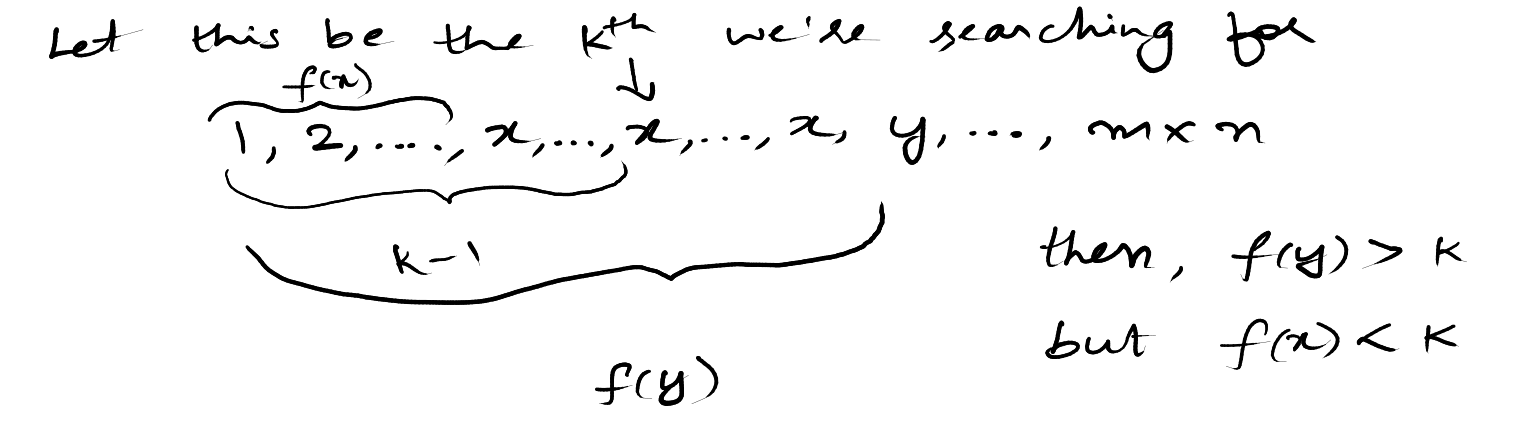
\includegraphics[scale=0.25]{cf448d}
\end{itemize}

\end{document}

